\documentclass{standalone}
\usepackage{tikz}

\begin{document}
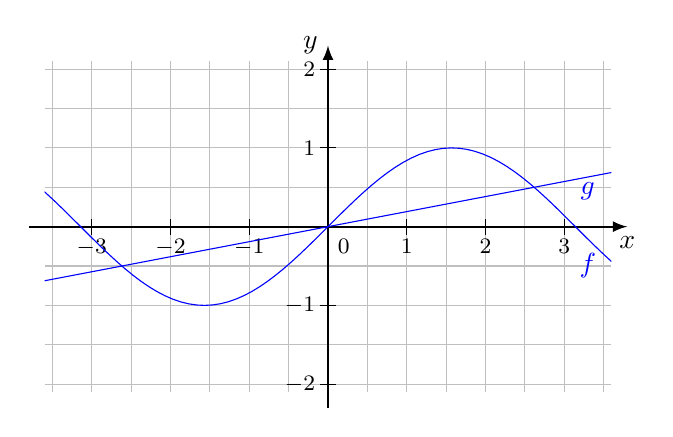
\begin{tikzpicture}[cross/.style={draw, cross out, minimum size=2*(#1-1pt), inner sep=0pt, outer sep=0pt}, x=10mm, y=10mm, 
    >=latex,   %Voreinstellung für Pfeilspitzen
    font= \footnotesize, scale=1]
    %Raster zeichnen
    \draw [color=gray!50]  [step=5mm] (-3.6,-2.1) grid (3.6,2.1);
    % Achsen zeichnen
    \draw[->,thick] (-3.8,0) -- (3.8,0) node[right, below] {\normalsize $x$};
    \draw[->,thick] (0,-2.3) -- (0,2.3) node[above, left] {\normalsize $y$};
    % Achsen beschriften
    \foreach \x in {-3,-2,-1,1,2,...,3} \draw (\x,-.1) -- (\x,.1) node[below=4pt] {$\x$};
    \foreach \y in {-2,-1,1,2} \draw (-.1,\y) -- (.1,\y) node[left=4pt] {$\y$};
    % Besserer Ursprung
    \draw[color=black] (0pt,-7pt) node[right] {$0$};
    %Funktionen zeichnen:
    \clip(-3.6,-2.1) rectangle (3.6,2.1); %Bildbereich
    \draw[blue,samples=100] plot (\x,{sin(\x r)});
    \draw[blue,samples=100] plot (\x,{0.190986*\x});
    %Beschriftung
    \node[blue]  at (3.3,-0.5) {\normalsize$f$};
    \node[blue]  at (3.3,0.45) {\normalsize$g$};
\end{tikzpicture}


\end{document}